\documentclass[a4paper, 12pt, twoside]{article}
\usepackage[T2A,T1]{fontenc}
\usepackage[utf8]{inputenc}
\usepackage[english, russian]{babel}
\usepackage{graphicx}
\usepackage[hcentering, bindingoffset = 10mm, right = 15 mm, left = 15 mm, top=20mm, bottom = 20 mm]{geometry}
\usepackage{multirow}
\usepackage{lipsum}
\usepackage{amsmath, amstext}
\usepackage{siunitx}
\usepackage{subcaption}
\usepackage{wrapfig}
\usepackage{adjustbox}
\usepackage{enumerate, indentfirst, float}
\usepackage{capt-of, svg}
\usepackage{ctable}
\usepackage{cmap} % Улучшенный поиск русских слов в полученном pdf-файле

\usepackage{pscyr} % Нормальные шрифты
\usepackage[normalem]{ulem} % для подчёркиваний uline
\ULdepth = 0.16em

\usepackage{fancyhdr} %Колонтикулы
\pagestyle{fancy}
\lhead{
\includegraphics[width = 10 mm]{logo.jpg} Лабораторная работа № 3.4.4}
\rhead{\textit{\today}}

\newenvironment{bottompar}{\par\vspace*{\fill}}{\clearpage}
 
\begin{document}
\begin{titlepage}

\newcommand{\HRule}{\rule{\linewidth}{0.7mm}} % Defines a new command for the horizontal lines, change thickness here

\center % Center everything on the page
 
%----------------------------------------------------------------------------------------
%	HEADING SECTIONS
%----------------------------------------------------------------------------------------

\textsc{\LARGE Московский Физико-Технический Институт}\\[1,5cm] % Name of your university/college
\textsc{\Large Кафедра общей физики}\\[0.5cm] % Major heading such as course name
\textsc{\large Лабораторная работа \textnumero  3.4.4}\\[0.5cm] % Minor heading such as course title

%----------------------------------------------------------------------------------------
%	TITLE SECTION
%----------------------------------------------------------------------------------------

\HRule
\\[0.4cm]
{ \huge \bfseries Петля гистерезиса \\(статистический метод).}
\\[0.2cm] % Title of your document
\HRule
\\[1.5cm]


 
%----------------------------------------------------------------------------------------
%	AUTHOR SECTION
%----------------------------------------------------------------------------------------

\begin{minipage}{0.4\textwidth}
	\begin{flushleft} \large
		\textbf{Автор:}\\
		Глеб Уваркин \\
		615 группа
	\end{flushleft}
\end{minipage}
~
\begin{minipage}{0.4\textwidth}
	\begin{flushright} \large
		\textbf {Преподаватель:} \\
		Андрей Александрович Заболотных % Supervisor's Name
	\end{flushright}
\end{minipage}

\begin{bottompar}
	\begin{center}
		
\includegraphics[width = 80 mm]{logo.jpg}
	\end{center}
	{\large \today}

\end{bottompar}
\vfill % Fill the rest of the page with whitespace

\end{titlepage}

{\Large \uline { \textbf  {Цель работы:}}}

\vspace{2mm}

Исследование кривых намагничивания ферромагнетиков с помощью баллистического гальванометра.

\vspace{\baselineskip}

{\Large \uline { \textbf  {В работе используются:}}}

\vspace{2mm}

Генератор тока с источником питания, тороид, соленоид, баллистический гальванометр с осветителем и шкалой, мультиметр-амперметр, лабораторный автотрансформатор(ЛАТР), разделительный трансформатор.

\section{Теоретические сведения.}
\subsection{Предмет исследования.}

\begin{wrapfigure}{r}{0.3\linewidth} 
	
	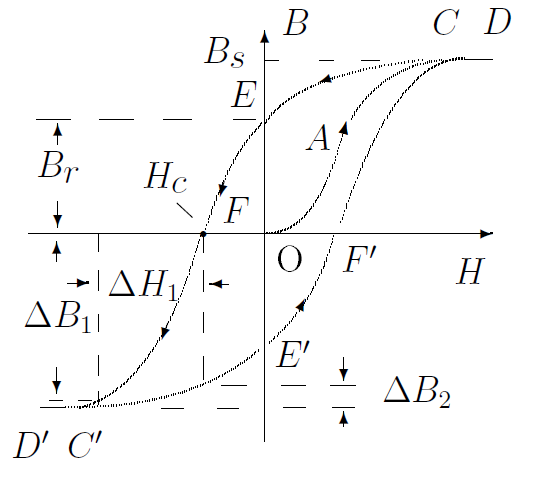
\includegraphics[width=\linewidth]{gist}
	\caption{Петля гистерезиса ферромагнетика.}
	\label{gist}
\end{wrapfigure}
К ферромагнетикам принадлежат железо, никель, кобальт, гадолиний, их многочисленные сплавы с другими металлами. К ним примыкают ферриты - диэлектрики со структурой антиферромагнетика.

Магнитная индукция \textbf{B} и напряженность магнитного поля \textbf{H} в ферромагнитном материале неоднозначно связаны между собой: индукция зависит не только от напряжённости, но и от предыстории образца. Связь между индукцией и напряжённостью поля типичного ферромагнетика иллюстрирует рис. \ref{gist}.
Здесь $B_s$ - индукция насыщения, величина $B_r$, достигаемая в точке $H = 0$ при возвращении из состояния насыщения, носит название \textit{остаточной индукции}. Значение $B = 0$ достигается лишь при некотором отрицательном значении $H = -H_c$. Величина $H_c$ называется \textit{коэрцитивной силой}.



\subsection{Основные формулы.}

Индукция \textbf{B} в образце состоит из индукции, связанной с намагничивающим полем \textbf{H}, и индукции, создаваемой самим намагниченным образцом. В системе СИ эта связь имеет вид
\begin{equation}
\textbf{B} = \mu_0(\textbf{H} + \textbf{M}),
\label{f1}
\end{equation}

где \textbf{M} - \textit{намагниченность} - магнитный момент единичного объёма образца, а $\mu_0$ - магнитная постоянная.

Кривая $OACD$, изображающая зависимость $B(H)$, практически совпадает с зависимостью $M(H)$, поскольку второй член в выражении (\ref{f1}) - в малых полях - существенно превосходит первый.

Напряжённость магнитного поля $H$ в тороиде зависит от тока, текущего в намагничивающей обмотке:
\begin{equation}
H = \dfrac{N_{T_0}}{\pi D}I,
\label{f2}
\end{equation}
где $D$ - средний диаметр тора.

Связь между отклонением зайчика в делениях ($\Delta x \sim \varphi$) и изменением магнитной индукции $\Delta x \sim B$ в сердечнике тороида:
\begin{equation}
\Delta B = \mu_0 \left (\dfrac{d_C}{d_T}\right )^2 \dfrac{R}{R_1} \dfrac{N_{C_0}}{N_{T_1}}\dfrac{N_{C_1}}{l_C}\Delta I_1 \dfrac{\Delta x}{\Delta x_1}
\label{f3}
\end{equation}
Формула (\ref{f3}) справедлива, если полные сопротивления измерительных цепей тороида и соленоида одинаковы: $R = R_1$.



Скорость подъёма кривой $OA$ характеризуется дифференциальной магнитной проницаемостью
\begin{equation}
\mu_{\text{диф}} = \dfrac{1}{\mu_0}\dfrac{dB}{dH}.
\end{equation}


\section{Экспериментальная установка.}

\begin{figure}[H]
	\centering
	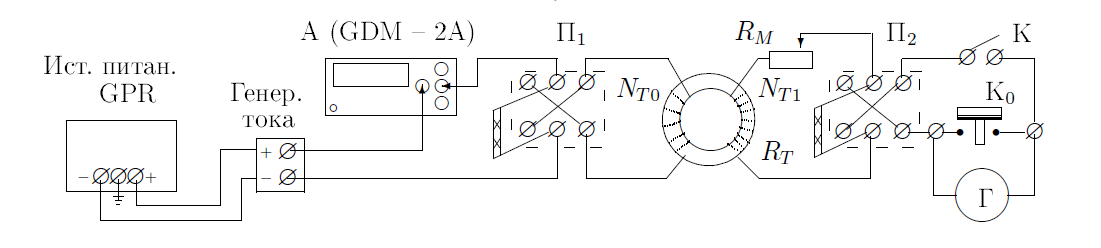
\includegraphics[width = \textwidth]{schem}
	\caption{Схема установки для исследования петли гистерезиса.}
	\label{schem}
\end{figure}

Схема для исследования петли гистерезиса представлена на рис. \ref{schem} . К источнику постоянного напряжения (GPR) подключён специальный генератор, позволяющий скачками менять токи в намагничивающей обмотке. Одинаковые скачки $\Delta I (\sim \Delta H)$ вызовут разные отклонения зайчика гальванометра $\Delta x (\sim \Delta B)$ на разных участках петли: на рис. \ref{gist} скачок $\Delta H_1$ может дать и $\Delta B_1$ на участке $FD^{'}$, и $\Delta B_2$ на участке $D^{'}E^{'}$. Поэтому генератор меняет ток неравномерно: большими скачками вблизи насыщения и малыми вблизи нуля.

Ток в намагничивающей обмотке измеряется цифровым мультиметром A. Переключатель $\Pi_1$ позволяет менять направление тока в первичной обмотке.

Чувствительность гальванометра $\Gamma$ во вторичной цепи можно менять с помощью магазина сопротивлений $R_M$. Ключ $K$ предохраняет гальванометр от перегрузок и замыкается только на время измерения отклонений зайчика. Ключ $K_0$ служит для мгновенной остановки зайчика (короткое замыкание гальванометра). Переключателем $\Pi_2$ можно изменять направление тока через гальванометр.

\begin{figure}[H]
	\centering
	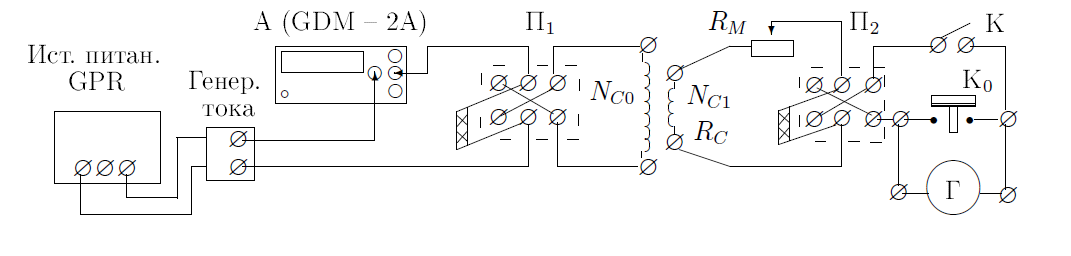
\includegraphics[width = \textwidth]{schem2}
	\caption{Схема установки для калибровки гальванометра.}
	\label{schem2}
\end{figure}

Схема на рис. \ref{schem2} отличается от схемы на рис. \ref{schem} только тем, что вместо тороида подключён калибровочный соленоид.

Сопротивление измерительных цепей тороида ($R = R_T+R_M+R_0$) и соленоида ($R_1 = R_C + R^{'}_M+R_0$) должны быть одинаковыми.

Сопротивление тороида $R_T \ll R_0$ - сопротивления гальванометра, поэтому сопротивления магазина в схеме с тороидом и соленоидом отличаются на величину сопротивления соленоида  $R_C: R^{'}_M = R_M - R_C$
\begin{figure}[H]
	\centering
	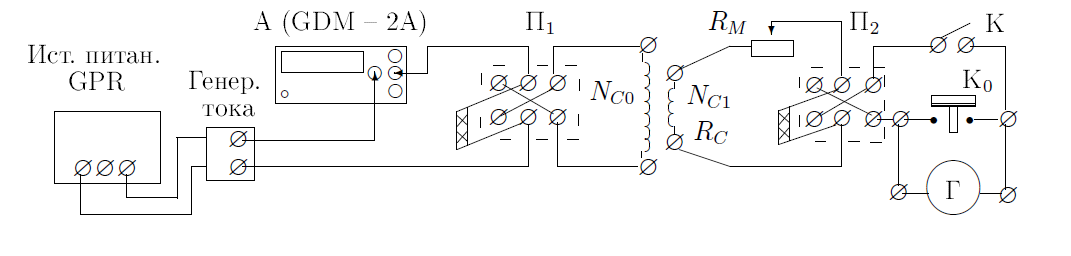
\includegraphics[width = \textwidth]{schem2}
	\caption{Схема установки для калибровки гальванометра.}
	\label{schem2}
\end{figure}




Чтобы снять начальную кривую намагничивания, нужно размагнитить сердечник. Для этого тороид подключается к цепи переменного тока (рис. \ref{schem3}). При уменьшении амплитуды тока через намагничивающую обмотку от тока насыщения до нуля характеристики сердечника \textbf{B} и \textbf{H} <<пробегают>> за секунду 50 петель всё меньшей площади и в итоге приходят в нулевую точку.
\begin{figure}[H]
	\centering
	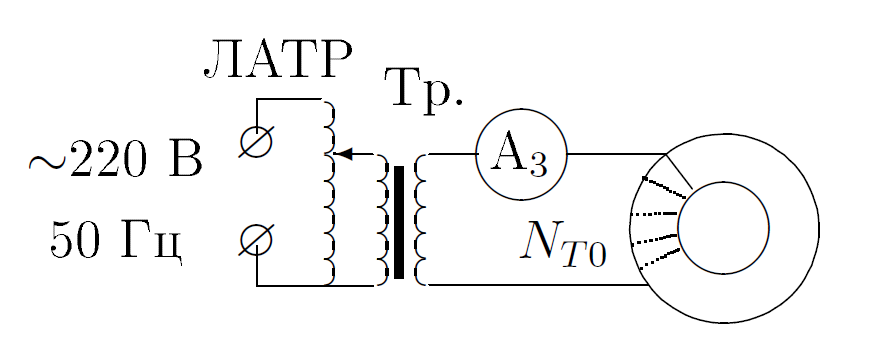
\includegraphics[width = 0.7\textwidth]{schem3}
	\caption{Схема установки для размагничивания образца.}
	\label{schem3}
\end{figure}

\textbf{Запишем параметры установки:}


\begin{minipage}{0.3 \linewidth}
	$N_{T_1} = 300$
	
	$N_{T_0} = 1750$
	
	$d_T = 1$ см
	
	$\Delta x_1 = 9.5$ см
	
	$D = 10$ см
	
\end{minipage}
~
\begin{minipage}{0.3 \linewidth}
	$R_C = 60$ Ом
	
	$N_{C_1} = 435$
	
	$N_{C_0} = 825$
	
	$l_C = 80$ см
	
	$d_C = 7$ см
\end{minipage}
~
\begin{minipage}{0.3 \linewidth}
	
	$R_0 = 50$ Ом
	
	$R_M = 75$ Ом
	
	$I_{max} = 1.472$ A
	
	$R_M^{'} = 15$ Ом
\end{minipage}

\newpage

\section{Обработка результатов.}

\begin{table}[H]
	\centering
	\caption{Петля гистерезиса(полученные значения).}
	\label{pet}
	\begin{tabular}{c|c|c|c|c|c|c|c|c|c}
		\toprule
		$I$, мА        & 1467 & 537   & 244.6 & 147.5 & 96.9  & 65.6  & 50.1  & 40.6               & 34.7              \\ 
		$\Delta x$, см & 12.6 & 12.9  & 9.2   & 6.9   & 5.4   & 3.1   & 2.1   & 1.3                & 0.7               \\ \midrule
		$I$, мА        & 31.7 & 27.9  & 24.2  & 1.1   & 0     & 1.1   & 24.3  & 27.9               & 31.7              \\ 
		$\Delta x$, см & 0.9  & 0.9   & 7.5   & 0.3   & 0.4   & 13    & 3     & 4.3                & 4.6               \\ \midrule
		$I$, мА        & 34.7 & 40.7  & 50.2  & 65.6  & 96.9  & 147.4 & 244.4 & 537.3              & 1468              \\ 
		$\Delta x$, см & 13   & 23.6  & 22.8  & 23.7  & 18.2  & 17    & 21.4  & 16.7               & 12.3              \\ \midrule
		$I$, мА        & 538  & 244.6 & 147.3 & 96.9  & 65.5  & 50    & 40.6  & 34.6               & 31.6              \\ 
		$\Delta x$, см & 12.5 & 9.1   & 6.7   & 5.4   & 3     & 2     & 1.3   & 0.7                & 0.9               \\ \midrule
		$I$, мА        & 27.8 & 24.2  & 1     & 0.2   & 1     & 24.1  & 27.8  & 31.6               & 34.6              \\ 
		$\Delta x$, см & 0.9  & 7.3   & 0.3   & 0.4   & 12.4  & 2.9   & 4     & 4.4                & 14.4              \\ \midrule
		$I$, мА        & 40.7 & 50.2  & 65.6  & 96.9  & 147.5 & 244.5 & 538   & \multicolumn{2}{c}{\multirow{2}{*}{}} \\ 
		$\Delta x$, см & 23.5 & 22.4  & 23.1  & 17.5  & 16.6  & 20.3  & 16.2  & \multicolumn{2}{c}{}                  \\ \bottomrule
	\end{tabular}
\end{table}

\begin{table}[H]
	\centering
	\caption{Начальная кривая намагничивания(полученные значения).}
	\label{nach}
	\begin{tabular}{c|c|c|c|c|c|c|c}
		\toprule
		$I$, мА        & 0    & 0.77 & 23.8 & 27.5  & 31.3  & 34.3 & 40.3 \\ 
		$\Delta x$, см & 0.1  & 4.6  & 1.4  & 1.8   & 1.7   & 4.1  & 6.9  \\ \midrule
		$I$, мА        & 49.8 & 65.2 & 96.5 & 147.2 & 244.3 & 537  &      \\ 
		$\Delta x$, см & 9.7  & 14.4 & 14.6 & 16.2  & 21    & 14.6 &      \\ \bottomrule
	\end{tabular}
\end{table}

С помощью таблиц \ref{pet} и \ref{nach}, а также формул (\ref{f2}) и (\ref{f3})
построим петлю гистерезиса $B = f(H)$. Ось $H(I)$ проведём через середину петли. На том же графике построим начальную кривую намагничивания (см. рис (\ref{graph})).

\begin{table}[H]
	\centering
	\caption{Зависимость B(H) для петли гистерезиса.}
	\label{zavg}
	\begin{tabular}{c|c|c|c|c|c|c|c|c|c}
		\toprule
		$H$, А/м & 8175  & 2992  & 1363  & 822   & 540   & 365   & 279   & 226   & \multicolumn{1}{c}{193}   \\ 
		$B$, Тл  & 1.73  & 1.55  & 1.37  & 1.24  & 1.14  & 1.06  & 1.02  & 0.99  & \multicolumn{1}{c}{0.97}  \\ \midrule
		$H$, А/м & 177   & 155   & 135   & 6     & 0     & -6    & -135  & -155  & \multicolumn{1}{c}{-177}  \\ 
		$B$, Тл  & 0.96  & 0.95  & 0.93  & 0.83  & 0.82  & 0.82  & 0.63  & 0.59  & \multicolumn{1}{c}{0.53}  \\ \midrule
		$H$, А/м & -193  & -227  & -280  & -366  & -540  & -822  & -1362 & -2995 & \multicolumn{1}{c}{-8182} \\ 
		$B$, Тл  & 0.46  & 0.28  & -0.06 & -0.39 & -0.72 & -0.98 & -1.23 & -1.53 & \multicolumn{1}{c}{-1.77} \\ \midrule
		$H$, А/м & -2998 & -1363 & -821  & -540  & -365  & -279  & -226  & -193  & \multicolumn{1}{c}{-176}  \\ 
		$B$, Тл  & -1.59 & -1.41 & -1.29 & -1.19 & -1.11 & -1.07 & -1.04 & -1.02 & \multicolumn{1}{c}{-1.01} \\ \midrule
		$H$, А/м & -154  & -135  & -6    & 0     & 6     & 134   & 155   & 176   & \multicolumn{1}{c}{193}   \\ 
		$B$, Тл  & -1.00 & 0.99  & -0.88 & -0.88 & -0.87 & -0.70 & -0.65 & -0.60 & \multicolumn{1}{c}{-0.53} \\ \midrule
		$H$, А/м & 227   & 280   & 366   & 540   & 822   & 1363  & 2998  & 8187  &                            \\ 
		$B$, Тл  & -0.33 & 0.01  & 0.33  & 0.65  & 0.90  & 1.14  & 1.43  & 1.66  &                            \\ \bottomrule
	\end{tabular}
\end{table}


\begin{table}[H]
	\centering
	\caption{Зависимость B(H) для начальной кривой намагничивания.}
	\label{zavn}
	\begin{tabular}{c|c|c|c|c|c|c|cc}
		\toprule
		$H$, А/м & 0     & 4.3   & 132.6 & 153.3  & 174.4  & 191    & \multicolumn{1}{c|}{224.6} & \multicolumn{1}{c}{277.5} \\ 
		$B$, Тл  & 0     & 0.001 & 0.067 & 0.087  & 0.113  & 0.137  & \multicolumn{1}{c|}{0.195} & \multicolumn{1}{c}{0.294} \\ \midrule
		$H$, А/м & 363.4 & 537.8 & 820.4 & 1361.5 & 2992.8 & 8192.7 & \multicolumn{2}{c}{\multirow{2}{*}{}}                   \\ 
		$B$, Тл  & 0.432 & 0.638 & 0.846 & 1.077  & 1.377  & 1.585  & \multicolumn{2}{c}{}                                    \\ \bottomrule
	\end{tabular}
\end{table}

\begin{figure}[H]
	\centering
	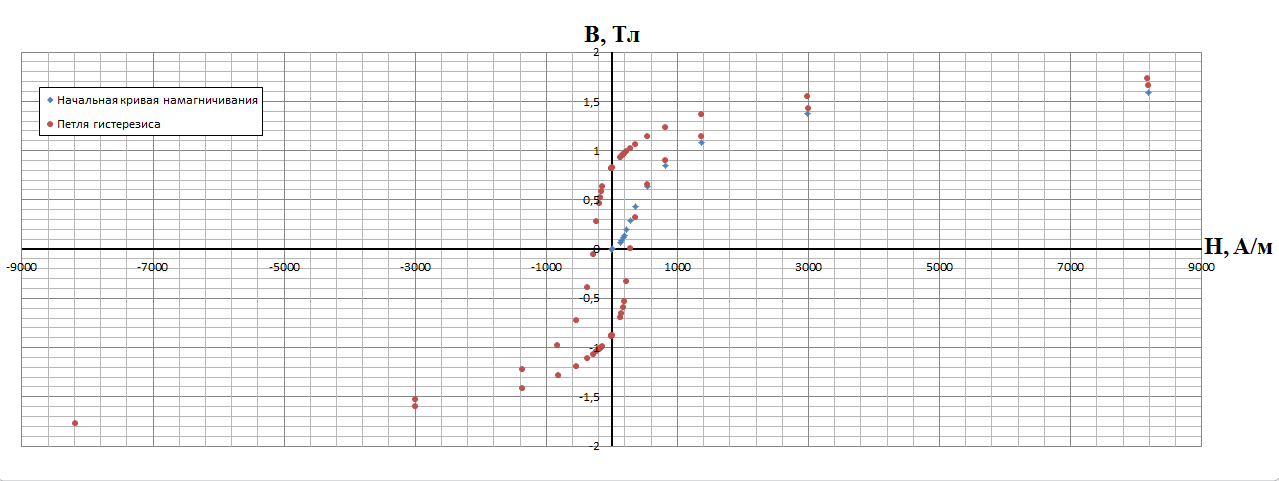
\includegraphics[width = \textwidth]{graph}
	\caption{Петля гистерезиса и начальная кривая намагничивания ферромагнетика(эксперимент).}
	\label{graph}
\end{figure}

Определим по графику коэрцитивную силу $H_c$ и индукцию насыщения $B_s$, а также максимальное значение дифференциальной магнитной проницаемости $\mu_{\text{диф}}$. Полученные значения занесём в таблицу \ref{itog}.

\begin{table}[H]
	\centering
	\caption{Итоговые значения.}
	\label{itog}
	\begin{tabular}{c|c|c}
		\toprule
		& Эксперим.  & Табличн. \\ \midrule
		$H_c$, А/м        & $270\pm 130$ &    $140$      \\ 
		$B_s$, Тл         & $1.733\pm 0.400$      & $2.12$         \\  
		$\mu_{\text{диф}}$ & $1479.5\pm 521$           & $2000$         \\ \bottomrule
		\end{tabular}
\end{table}

\section{Вывод.}

Было исследовано явление гистерезиса на примере образца стали. Полученная петля очень близка к теоретической. Были оценены значения коэрцитивной силы $H_c$, индукции насыщения $B_s$ и максимальное значение дифференциальной магнитной проницаемости $\mu_{\text{диф}}$. 

Погрешность получилась достаточно большой ($\varepsilon_{\text{\tiny{\text{$H_c$}}}} \approx 50\%$, $\varepsilon_{\text{\tiny{\text{$B_s$}}}} \approx 23\%$, $\varepsilon_{\text{\tiny{\text{$\mu_{\text{диф}}$}}}} \approx 35\%$). Это можно объяснить несовершенством метода измерений - достаточно сложно уловить отклонения "зайчика" с большой точностью, а в окрестности $H = 0$ отклонения составляли всего лишь доли сантиметра. Также сюда можно приписать устаревшее оборудование и влияние внешних электронных устройств.




\end{document}